% !TEX encoding = UTF-8 Unicode
\documentclass{article}

\usepackage{polski}
\usepackage[utf8]{inputenc}
\usepackage{subfig}
\usepackage{multirow}
\usepackage{graphicx}

\usepackage[a4paper, left=2.5cm, right=2.5cm, top=3.5cm, bottom=3.5cm, headsep=1.2cm]{geometry}

\linespread{1.3}
\begin{document}
	
	\begin{titlepage}
		\centering
		{\scshape\LARGE Politechnika Wrocławska \par}
		{\scshape\Large Katedra Informatyki Technicznej\par}
		
		\vspace{1cm}
		{\scshape\Large Inżynieria Oprogramowania\par}
		\vspace{1.5cm}
		{\huge\bfseries Specyfikacja wymagań funkcjonalnych za pomocą diagramu przypadków użycia\par}
		\vspace{2cm}
		{\Large\itshape Magdalena Biernat\par}
		{\Large\itshape Mateusz Bortkiewicz\par}
		\vfill
		Opiekun\par
		prof. dr hab. inż. Jan Magott 
		
		\vfill
		{\large \today\par}
	\end{titlepage}
	\newpage
	
	\section{Wprowadzenie}
	Sprawozdanie dotyczy trzecich i czwartych zajęć. Na tych laboratoriach zaczęliśmy swój projekt. 
	
	\subsection{Cel laboratorium}
Specyfikacja wymagań, zdefiniowanych w ramach laboratorium 2, za pomocą diagramów przypadków użycia – tworzenie modelu
przypadków użycia 
	
	\subsection{Plan pracy}
	Zadania wykonaliśmy wg instrukcji 3:

	\begin{itemize}
		\item Wykonanie diagramu przypadków użycia.
		\item Zdefiniowanie aktorów.
		\item Wykonanie scenariuszy przypadków użycia.
	\end{itemize}

	\section{Laboratorium}
	\subsection{Wykonanie diagramu przypadków użycia}
	\begin{figure}[!ht]
	\centering
	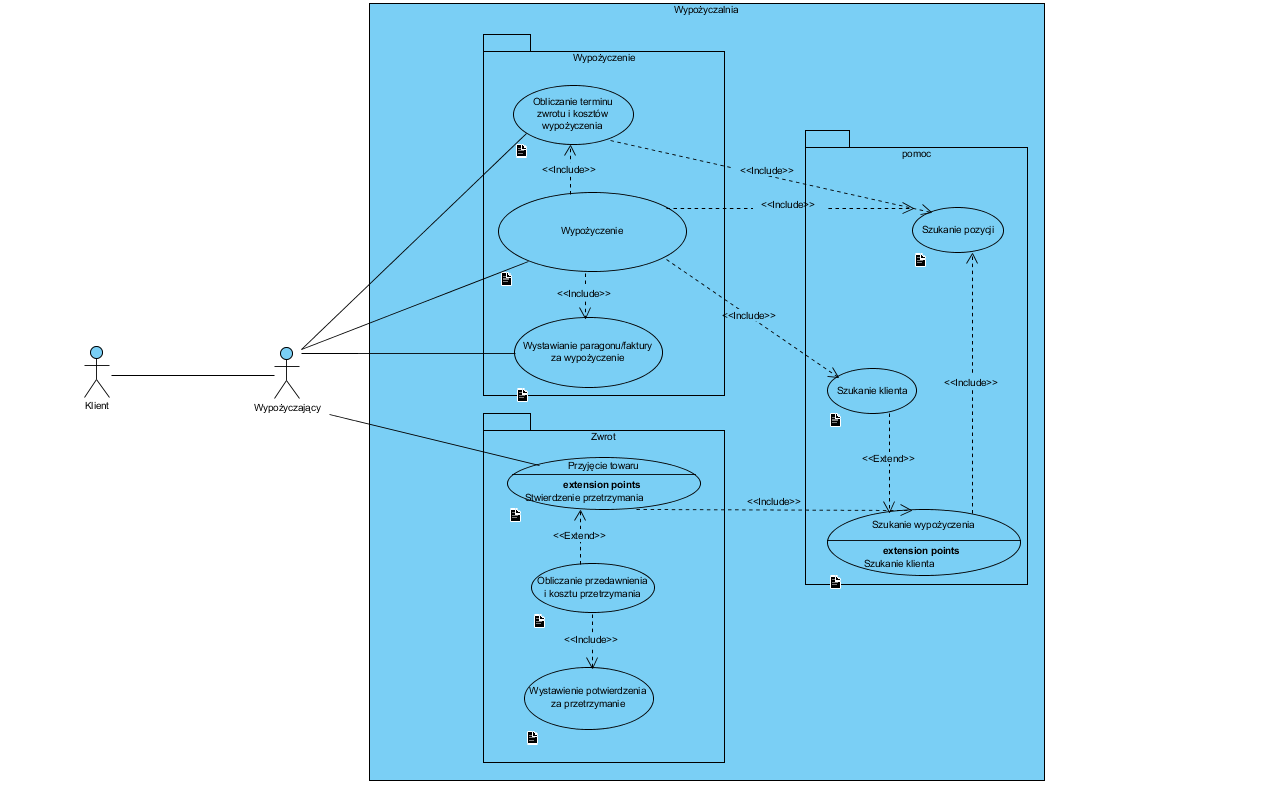
\includegraphics[height=10cm]{diagram.png}
	\caption{Stworzony diagram przypadków użycia}
	\label{fig:obrazek 1}
	\end{figure}
	\subsection{Zdefiniowanie aktorów}
	
\begin{tabular}{| p{2,5cm} | p{6,5cm} | p{6cm} |} \hline 
	AKTOR & OPIS & PRZYPADKI UŻYCIA   \\ \hline
	\multirow{3}{*}{Klient} & Klient wypożycza za pośrednictwem wypożyczającego & 
	Obliczanie terminu zwrotu i kosztów wypożyczenia \par
	Wypożyczenie \par
	Wystawienie paragonu/faktury za wypożyczenie \\ 
	\hline
	\multirow{5}{*}{Wypożyczający} & Wypożyczający wypożycza klientowi towar korzystając z aplikacji.  Aplikacja wylicza termin i koszt wypożyczenia Może też wyszukiwać klienta i artykuły. Może też wystawić rachunek lub fakturę. Wypożyczający przyjmuje również zwroty i aplikacja wylicza wtedy przedawnienie i koszt przetrzymania. & Przyjęcie towaru\par
	Obliczenie przedawnienia i kosztu przetrzymania\par
	Szukanie pozycji\par
	Szukanie klienta\par
	Szukanie wypożyczenia \\ \hline
\end{tabular}
\subsection{Wykonanie scenariuszy użycia}	
\subsubsection{Wypożyczenie: Obliczanie terminu zwrotu i kosztów wypożyczenia}
\begin{enumerate}
	\item [Cel:] Obliczenie terminu zwrotu i kosztów wypożyczenia na podstawie informacji od klienta i wskazanych pozycji.
	\item [WS:] Może być wywołany przez Wypożyczającego, musi być wywołany przy Wypożyczeniu
	\item [WK:] Podanie terminu zwrotu i kosztów wypożyczenia
	\item [Przebieg:]
	\begin{enumerate}
	\item [1.]Odwołanie się do produktu w bazie danych
	\item [2.]Zwrot terminu i kosztów wypożyczenia na podstawie danych produktu
	\end{enumerate}
\end{enumerate}

\subsubsection{Wypożyczenie: Wypożyczenie}
\begin{enumerate}
	\item[Cel:] Wypożyczenie klientowi produktu/produktów. 
	\item[WS:] Produkt musi być niewypożyczony 
	\item[WK:] Wypożyczenie musi być zarejestrowane w systemie
	\item[Przebieg:]
	\begin{enumerate}
		\item [1.]Szukamy klienta.
		\item [2.]Następuje obliczenie terminu zwrotu i kosztów wypożyczenia.
		\item [3.]Klientowi zostają przypisane pozycje – następuje wypożyczenie
		\item [4.]Następuje wystawienie paragonu/faktury za wypożyczenie.
	\end{enumerate}
\end{enumerate}

\subsubsection{Wypożyczenie: Wystawienie paragonu/faktury za wypożyczenie}
\begin{enumerate}
	\item[Cel:] Wystawienie klientowi paragonu/faktury
	\item[WS:] Wypożyczenie musi być zarejestrowane w systemie
	\item[WK:]  Paragon/faktura musi być zarejestrowana w systemie.
	\item[Przebieg:]
	\begin{enumerate}
		\item [1.]Na podstawie danych z wypożyczenia jest generowany dokument
		\item [2.]Dokument jest zapisany do systemu
	\end{enumerate}
\end{enumerate}

\subsubsection{Zwrot: Przyjęcie towaru}
\begin{enumerate}
\item[Cel:] Zwrot wypożyczonego uprzednio towaru
	\item[WS:] Towar musi być wypożyczony
	\item[WK:]  Towar będzie dostępny do wypożyczenia, a klient rozliczony z wypożyczalnią.
	\item[Przebieg:]
	\begin{enumerate}
		\item [1.]Znalezienie wypożyczenia na podstawie wypożyczonej pozycji.
		\begin{enumerate}
			\item [1.1] Opcjonalnie za pomocą danych klienta 
		\end{enumerate}
		\item [2.]Jest wystawione potwierdzenie zapłaty za przetrzymanie
			\begin{enumerate}
			\item [2.1] Opcjonalnie za pomocą danych klienta 
		\end{enumerate}
		\item [3.]Towar jest zwrócony do wypożyczalni.
	\end{enumerate}
\end{enumerate}

\subsubsection{Zwrot: Obliczanie przedawnienia i kosztu przetrzymanie}
\begin{enumerate}
	\item[Cel:] Obliczanie przedawnienia i kosztów przetrzymania
	\item[WS:] Termin wypożyczenia musi być przekroczony
	\item[WK:]  Wystawienie potwierdzenia zapłaty za przetrzymanie wypożyczalnią.
	\item[Przebieg:]
	\begin{enumerate}
		\item [1.]Pobierana jest przetrzymana pozycja i w zależności od niej – obliczana kwota przetrzymania
		\item [2.]Następuje generowanie dokumentu
		\item [3.] Dokument jest zapisany do systemu
	\end{enumerate}
\end{enumerate}
	
\subsubsection{Zwrot: Wystawienie potwierdzenia za przetrzymanie}
	\begin{enumerate}
		\item[Cel:] Wystawienie potwierdzenia za przetrzymanie
		\item[WS:] We wskazanym wypożyczeniu musi wystąpić przedawnienie
		\item[WK:] Wystawienie potwierdzenia zapłaty za przetrzymanie
		\item[Przebieg:]
	\begin{enumerate}
		\item [1.]Zostaje pobrany termin i kwota przedawnienia 
		\item [2.]Następuje generowanie dokumentu
		\item [3.]Dokument jest zapisany do systemu
	\end{enumerate}
	\end{enumerate}
	
\subsubsection{Pomoc: Szukanie wypożyczenia}
\begin{enumerate}
	\item[Cel:] Wyszukanie interesującego nas wypożyczenia
	\item[WS:] Musi zostać wprowadzona dana do wyszukiwania: np. tytuł, kod kreskowy etc albo dana klienta
	\item[WK:] Zwrócona zostaje interesujące nas wypożyczenie
	\item[Przebieg:]
\begin{enumerate}
	\item [1.]Zostaje zeskanowany kod kreskowy 
	\begin{enumerate}
		\item [1.1] Jeśli jest nieczytelny to wyszukujemy dane klienta
	\end{enumerate}
	\item [2.]Jeśli pozycja jest niewypożyczona, zwracamy informację o braku wypożyczenia
	\item [3.]Jeśli jest wypożyczona, to zwracamy wypożyczenie.
\end{enumerate}
\end{enumerate}

	\subsubsection{Pomoc: Szukanie klienta}
	\begin{enumerate}
		\item[Cel:] Wyszukanie klienta
		\item[WS:] Musi zostać wprowadzona dana klienta: Nazwisko, Pesel albo telefon
		\item[WK:] Zwrócenie konta klienta
		\item[Przebieg:]
	\begin{enumerate}
		\item [1.]Zostaje pobrana dana
		\item [2.]Jeśli brak takiego klienta, zwracamy informację o braku konta
		\item [3.]Jeśli występuje klient to zwracamy jego konto
	\end{enumerate}
	\end{enumerate}
	
	\subsubsection{Pomoc: Szukanie pozycji}
	\begin{enumerate}
		\item[Cel:] Wyszukanie pozycji, instancji tytułu artykułu
		\item[WS:] Musi zostać wprowadzona dana do wyszukiwania: Kod kreskowy, nazwa albo autor
		\item[WK:] Zwrócenie interesującej nas pozycji
		\item[Przebieg:]
	\begin{enumerate}
		\item [1.]Zostaje pobrana dana
		\item [2.]Na podstawie danej zwracamy pasującej do niej pozycje książek
		\begin{enumerate}
		\item [2.1] Jeśli brak pozycji to zwracamy informację o braku pozycji
		\end{enumerate}
	\end{enumerate}
	\end{enumerate}

\end{document}